% Author: Henry Sun
% Email: tigerhs1998@berkeley.edu
\qns{Revisiting Touchscreens}

\sol{Ensure that students are familiar with series and parallel equivalences. Also, this question does not directly involve measuring height and position from resistor values}
\begin{center}
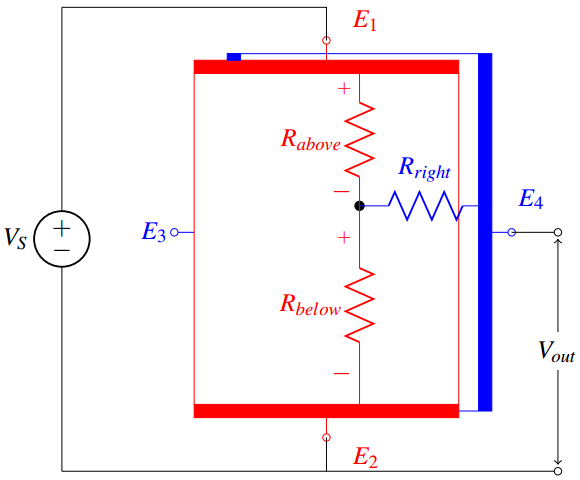
\includegraphics{../../questionBank/week06/q_touchscreen_figs/touchscreenpic.png}

Model of resistive touchscreen. Source: Note 11
\end{center}

In this question, we'll be re-examining the properties of the 2-dimensional resistive touchscreen introduced in class. First off, recall that we are modeling our touchscreen as a bunch of horizontal resistors in a mesh that can bend when touched, overlaying a large number of vertical resistors, forming a mesh underneath. When one resistor is pressed down, we can model the effects as so:
\begin{center}
\begin{circuitikz}
\draw(0,0) 
to [short] (0,1)
to [generic=$R_0$] (0,3)
to [short] (0,4);
\end{circuitikz}
$\Rightarrow$ When touched, becomes $\Rightarrow$
\begin{circuitikz}
\draw(2,0)
to [generic=$R_1$] (2,2)
to [short, l^=$Y$] (2,2)
to [generic=$R_2$] (2,4);


\end{circuitikz}
\end{center}

(Recall $R = \frac{\rho l}{A}$)

Since resistance is proportional to length, our position can be tracked by the value of the resistance! And since, by the voltage divider, voltage $V_y$ should equal

$$\frac{R_1}{R_1+R_2}$$

In other words, our voltage, our measurement, is directly related to our position!

\begin{enumerate}
\qitem{Say we have an initial resistor of length $l$ and cross sectional area $A$, with resistivity $\rho$. Say the resistor is touched at point Y. What are the resistances of $R_1$ and $R_2$? What is the value of their sum?}

\ans{The effective length of resistor $R_1$ is $Y$, and the effective length of resistor $R_2$ is $l - Y$. Since $\rho$ and $A$ are the same as from the original full length resistor $R_0$, these values remain the same. Thus we have:

$$R_1 = \frac{\rho Y}{A}, R_2 = \frac{\rho (l-Y)}{A}$$
$$ R_1 + R_2 = \frac{\rho (l-Y) + \rho Y}{A} = \frac{\rho l}{A} = R_0$$

The sum remains the same as the whole value! This is important for the next part.}

\qitem{Say we wanted to measure two simultaneous touches at $Y_1$ and $Y_2$. Assuming we can measure two output voltages, $V_{o1}$ and $V_{o2}$, what are the values of these voltages? Say we keep our finger down on $Y_1$, but release $Y_2$. Does the voltage $V_{o1}$ change? (This is the same thing as asking whether or not touching at $Y_2$ would affect the output voltage, and thus the reported height changes}
\begin{center}


\begin{circuitikz}
\draw(0,0)
to [R=$R_1$] (0,2)
to [short, l^=$Y_1$] (0,2)
to [R=$R_2$] (0,4)
to [short, l^=$Y_2$] (0,4)
to [R=$R_3$] (0,6);

\draw(0,2)
to [short, l^=$V_{o1}$] (1,2);

\draw(0,4)
to [short, l^=$V_{o2}$] (1,4);

\draw(0,6)
to [short] (-3,6)
to [short] (-3,3)
to [V=$V_s$] (-3,1)
to[short] node[ground] {} (-3,0)
to [short] (0,0);

\end{circuitikz}
\end{center}
\ans{First looking at $V_{o1}$, we can use our handy voltage divider equation! We know the resistor below is $R_1$, and above is, by series resistance, $R_2 + R_3$. Thus, 

$$V_{o1} = V_s\frac{R_1}{R_1+(R_2+R_3)}$$

Similarly for $V_{o2}$, we have the equivalent series resistance below as $R_1 + R_2$, and

$$V_{o2} = V_s\frac{R_1 + R_2}{(R_1+R_2)+R_3}$$

What if we were to lift up our finger at $Y_2$? Well, from part a), we know that the full length resistor $R_{23}$ (the equivalent resistor if did not touch at $Y_2$), will be the same value as $R_2 + R_3$. So, in fact, 

$$V_{o1} = V_s\frac{R_1}{R_1+R_{23}} = V_s\frac{R_1}{R_1+(R_2+R_3)}$$

Which is the same as before! In other words, touching in multiple places should not affect our original measurement, and thus could accurately measure the position of our touch!}

\qitem{Now, in the original model in class for the 2-D touchscreen, we ensured that the two meshes, the horizontal and vertical, were not powered at the same time. What happens, however, if we were to power both meshes at the same time? The equivalent circuit is shown below. Find the new, if at all, $V_{o}$ produced in this scenario. Would this be an accurate, overestimate, or underestimate of the height from ground?}


\begin{center}
\begin{circuitikz}
\draw(0,4)
to [short] (0,2)
to [V=$V_s$] (0,1)
to [short] node[ground] {} (0,0)
to [short] (2,0)
to [R=$R_2$] (2,2)
to [R=$R_1$] (2,4)
to [short] (0,4);

\draw(0,2)
to [R=$R_3$] (2,2)
to [R=$R_4$] (4,2)
to [short, l_=$V_{o}$, *-*] (4,2);

\draw(2,0)
to [short, *-*] (4,0);
\end{circuitikz}
\end{center}

\ans{First, notice that $R_4$ is sort of suspended, without any connections. Open, unconnected wires will have no current going through them, so the difference in voltage across $R_4$ is zero. So we can disregard this resistor.

Let's also redraw the circuit a bit, like so:

\begin{center}
\begin{circuitikz}
\draw(0,5)
to [short] (0,2)
to [V=$V_s$] (0,1)
to [short] node[ground] {} (0,0)
to [short] (2,0)
to [R=$R_2$] (2,2)
to [short] (1,2)
to [R=$R_3$] (1,4)
to [short] (2,4)
to [short] (2,5)
to [short] (0,5);

\draw(2,4)
to [short] (3,4)
to [R=$R_1$] (3,2)
to [short] (2,2);

\draw(3,2)
to [short, l^=$V_{o}$, *-*] (4,2);
\end{circuitikz}
\end{center}

Our new configuration has this interesting parallel configuration. Let's calculate $V_o$ here:

$$V_o = \frac{R_2}{R_2 + (R_1 || R_3)} \neq \frac{R_2}{R_2 + R_1}$$

So, as a matter of fact, it's incredibly important that our circuits stay separate! 

Since a parallel configuration is ALWAYS less than EITHER of the original resistor values, we'll in fact end up with a HIGHER voltage than expected, and thus we'll report a position higher up than we really touched!
}

\qitem{
\textbf{Extra Practice:}
Let's hone our design skills a bit. Think about the following design criteria needed for a real touch screen, and write down some ideas as to how to implement them, and see whether or not we can extend our resistive model to handle these elements. (Since we haven't gone over many circuit elements, this will be a high-level question, but good to get some design thinking going):

\begin{enumerate}
\item 3-D touchscreen. Is this feasible? Think about scaling up from the 2-D model. Can we actually "touch" at a point in space?


\item Swiping. What extra parameter do we have to consider in this case, besides just position?

\item Long touch-hold. Similar to above.
 
\end{enumerate}
}
\ans{
\begin{enumerate}
\item Probably not feasible. Remember, we're using overlaid meshes as our resistive model. To have 3 dimensions would require almost a solid cube of resistors! We'd need a different kind of model here.

\item The most important parameter now is that we have to consider time. In our model, we're likely switching between voltage sources many, many, many times per second to get thousands of measurements. Perhaps the best way to measure swiping is to measure the rate of change of $V_0$ over time, and if it exceeds a certain threshold, we activate the swipe command.

\item Same, but exact opposite as above. We'd want to see if our voltage $V_0$ stays constant over a period of time.

\end{enumerate}



}


\end{enumerate}
